\documentclass[a4paper,12pt]{report}
\usepackage[utf8]{inputenc}
\usepackage[colorlinks=true]{hyperref}
\usepackage{algorithmicx}
\usepackage{algorithm}
\usepackage{algpseudocode}
\usepackage{mathtools}
\usepackage{graphicx}
\usepackage{caption}
\usepackage{subcaption}
\usepackage{listings}
\usepackage{spverbatim}
\usepackage{geometry}
\usepackage{pdflscape}

% Title Page
\title{Optical Character Recognition Using ANN \& R}
\author{Jaishankar-13030142017}
\date{}


\begin{document}
\maketitle

\tableofcontents{}

\begin{abstract}
\addcontentsline{toc}{section}{Abstract}
This project aims to show basic workings of character recognition using Artificial Neural Networks (ANN) implemented in the R programming language.
Artifical Neural Networks are used widely in various fields of computer science, one of them being optical character recognition.
Artificial Neural Networks provide efficient solutions to complex problems which otherwise require high computational power. \\

\textbf{Why R??}\\

The R programming language is a powerful language that is used in statitstical and data analysis. The language provides a fast and easy 
handling of large data. Many of the matrix manipulations and other vector manipulations are a breeze. 
The combination of using ANN and R provides a very powerful platform for doing optical character recognition. 
This project delves into the very basics of optical character recognition.


\end{abstract}

\section*{Requirements}
\addcontentsline{toc}{section}{Requirements}
\begin{itemize}
 \item R v2.15.1 or greater
 \item R Packages required
  \begin{itemize}
   \item \verb+gWidgets+
   \item \verb+gWidgetsRGtk2+
   \item \verb+pixmap+
   \item \verb+stringr+
   \item \verb+RGtk2+
   \item \verb+RCpp+
   \item \verb+RSNNS+
    \item \verb+RStudio+ (Optional)
  \end{itemize}
  \vskip 1cm
  
  All these packages can be installed from the R repository using\\ \verb+install.packages(package_name)+. Also please do install all the dependency associated with any of them.
  
  R can be downloaded from \url{http://cran.r-project.org/bin/windows/base/} \& installed on your machine. For correct results please follow
  the install instructions for your operating system. 
  
  In this document the base operating system used is Open Suse 12.3. Any commands used are in reference to this os.

\end{itemize}

\pagebreak

\section*{Introduction}
\addcontentsline{toc}{section}{Introduction}
Optical Character Recognition or usually abbreviated to OCR is the mechanical or electronic conversion of text in images into computer-readable
format. This can later be modified or used as normal text in a computer. Actual OCRs perform a lot of tasks before performing actual character
recognition. i.e De-Skew, Despeckle, Binarization, Line Removal, Layout Analysis, Line \& Word detection...etc \cite{wikiocr}
The OCR that is presented in this document is a very very simple OCR, that takes an image of 9*9 pixel image that is in \verb+.pgm+ format.
This format is used because it can easily be converted into a binary representation for training the Neural networks.

\section*{A Brief Introduction to ANN}
\addcontentsline{toc}{section}{Brief Introduction to ANN}
In computer science ANN are mathematical models that are primarily inspired from the biological networks found in animal and human brains. 
This system constitutes a set of interconnected ``neurons'' that perform simple calculations.
The neuron sums up of all its inputs and produces an output if the amount of net input supplied is sufficient to activate it. (according to its activation function)
A system of these neurons is also called a neural network. Neural, because the whole idea is similar to the way the brain functions.
Usually the network constitutes of three layers, an input layer, an output layer and a hidden layer. The input layer receives the input,
the output layer produces the output of the net and the hidden layer performs most of the simple calculations.
Every connection between two neurons is associated with a weight. 

There are two phases to the functioning of the network. The first phase is known as the learning phase, and the second phase is known as the prediction phase.
In the learning phase the network is presented with a set of inputs known as training inputs, with their corresponding outputs known as targets.
The network learns to recognise these inputs with their corresponding outputs. Only when the network has completely learnt all the training inputs, the training phase 
is completed. The network presents its inputs to the hidden layer which performs the basic summation and activation and forwards its output to the output layer.
The output layer too performs its summation and activation and finally produces the output of the net. This output is compared with the corresponding target, and
the error is thus calculated. If the error is too high then the network has to continue learning. 

\begin{figure}[h!]
\centering
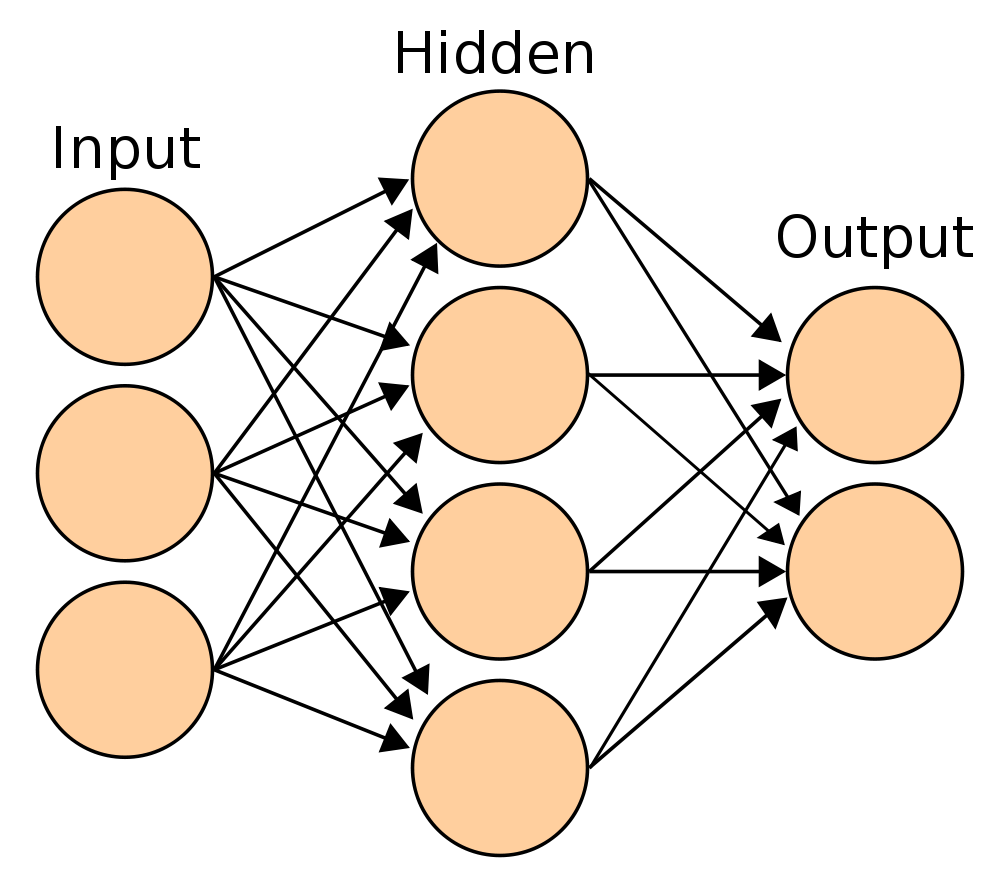
\includegraphics[width=\linewidth]{annnetwork.png} 
\caption{ANN Network\cite{fig1}}
\end{figure}



During learning the network performs some simple manipulations, the net basically calculates and updates the weights of the net. The calculation of the weight update is given by several different 
procedures also known as learning rules. The learning rule defines how the weights of the network need to be updated. There are two type of learning that can occur in a neural net.
One of them is known as the supervised learning rule, and the other is the unsupervised learning rule.

\subsubsection*{Supervised Learning}
\addcontentsline{toc}{subsection}{Supervised Learning}
Supervised learning refers to the fact that the net knows what to achieve during the training, or rather it is provided with the correct target to achieve.
Each training input has a corresponding target that is provided to the net. The net after having learnt to correspond each of the given inputs with their
corresponding target, tries to generalise to situations where the input is different from that of the training set.

\subsubsection*{UnSupervised Learning}
\addcontentsline{toc}{subsection}{Unsupervised Learning}
This kind of learning is opposite to that of the supervised learning. There are no specified targets provided to the network. The network based on the inputs
tries to classify and cluster inputs together. Many techniques like the Density estimation and Bayesian methods are used. The unsupervised learning is also as important if not more.
In this paper, only supervised learning is considered.

Following are few of the learning rules are discussed: 
\subsubsection*{Hebbian Learning Rule}
\addcontentsline{toc}{subsection}{Hebbian Learning Rule}
This is one of the earliest and simplest learning rule. This rule was proposed by Donald Hebb. Hebb proposed that learning occurs by modification of the weights
in a manner such that if two interconnected neurons are both ``on'' at the same time, then the weight between those neurons should be increased.

\addcontentsline{toc}{subsubsection}{Hebbian Algorithm}
The Algorithm can be summarised\cite{bookann}:
\begin{algorithm}[h!]
\caption{Hebbian Learning Rule}
\label{Hebbian Learning Rule}
\begin{algorithmic}
 \State Intialise all the weights:
      \State\hspace{\algorithmicindent} $w_i = 0$ 	($i = 1\ to\ n$)
 \For{each training pair $s : t$}:
      \State Set activations for input units:
	    \State\hspace{\algorithmicindent} $x_i = s_i$	($i = 1\ to\  n$)
      \State Set activation for output unit:
	    \State\hspace{\algorithmicindent} $y = t$	
      \State Adjust the weights for
	    \State\hspace{\algorithmicindent} $w_i(new) = w_i(old) + x_iy$ 	($i = 1\ to\ n$)
      \State Adjust the bias
	    \State\hspace{\algorithmicindent} $b_i(new) = b_i(old) + y$ 
  \EndFor
\end{algorithmic}
\end{algorithm}



\subsubsection*{Perceptron Learning Rule}
\addcontentsline{toc}{subsection}{Perceptron}
Perceptron perhaps had the most far reaching impact of any of the early neural nets. The perceptron learning rule is a more powerful 
learning rule than that of Hebb. Under some suitable conditions and assumptions, its iterative learning procedure can be proved to converge 
to the correct weights, the weights that allow the net to produce the correct output. This is a strong guarantee that the perceptron learning rule convergence theorem
provides us with, it can find the satisfactory weights for any problem in a limited number of iterations. There is a slight catch to that, the assumption is that such weights must exist.


\addcontentsline{toc}{subsubsection}{Perceptron Algorithm}
\begin{algorithm}[h!]
\caption{Perceptron Learning Rule}
\label{Perceptron Learning Rule}
The Algorithm can be summarised\cite{bookann}:\\
\begin{algorithmic}[h!]
 \State Intialise all the weights and bias:
      \State\hspace{\algorithmicindent} $w_i = 0$ 	($i = 1\ to\ n$)\\
 \State Intialise Learning rate $\alpha (0 < \alpha \leq 1)$ :
      \State\hspace{\algorithmicindent} (For Simplicity $\alpha$ can be set to 1).\\
 \While{Stopping condition is false}:\\
 \For{each training pair $s : t$}:
      \State Set activations for input units:
	    \State\hspace{\algorithmicindent} $x_i = s_i$	($i = 1\ to\  n$)
      \State Compute response of output unit:
	    \State\hspace{\algorithmicindent} $y_{in} = b + \sum\limits_i x_iw_i$;\\
	   \State \[ y = \left\{
		\begin{array}{l l}
		  1 & \quad \text{if $y_{in} > 0$}\\
		  0 & \quad \text{if $-\theta \leq y_{in} \leq \theta$}\\
		  -1 & \quad \text{if $y_{in} < 0$}
		\end{array} \right.\]\\ \\
      \State Adjust the weights and bias if an error occured:
	    \If{$y \neq t$},\\
		\hspace{\algorithmicindent}\hspace{\algorithmicindent}\hspace{\algorithmicindent}$w_i(new) = w_i(old) + \alpha tx_i$ \\
		\hspace{\algorithmicindent}\hspace{\algorithmicindent}\hspace{\algorithmicindent}$b_i(new) = b_i(old) + \alpha t$ \\
	    \Else,\\
		\hspace{\algorithmicindent}\hspace{\algorithmicindent}\hspace{\algorithmicindent}$w_i(new) = w_i(old)$\\
		\hspace{\algorithmicindent}\hspace{\algorithmicindent}\hspace{\algorithmicindent}$b_i(new) = b_i(old)$\\
	    \EndIf
  \EndFor
 \EndWhile
\end{algorithmic}
\end{algorithm}
\clearpage
\subsubsection*{Delta Learning Rule}
\addcontentsline{toc}{subsection}{Delta Learning Rule}
The Delta Learning rule also known as the (LMS) Least Mean Square rule, or the Widrow-Hoff rule. This learning rule minimizes the mean 
squared error between the activation and the target output. This rule is similar in other aspects to the other rules, except in the weight updation part.
This rule is a special case of the more general backpropagation rule.
\\ \\
The Error Calculation is given by:\\ \\
$E = \sum\limits_{j=1}^m (t_j - y\textunderscore in_j)^2$\\ \\
The weight updation is given by:\\ \\
$\Delta w_{IJ} = \alpha (t_J - y\textunderscore in_J)x_I.$ \\

\subsubsection*{Backpropagation}
\addcontentsline{toc}{subsection}{Delta Learning Rule}
Backpropagation is another learning procedure or rule that is very very powerful and can solve several problems that the other learning
rules fail to solve. It is a direct generalisation of the delta learning rule. This rule is not directly implemented in this paper, but 
a ready made package is used instead. (RSNNS)


\section*{Pattern Classification and Pattern Association}
\addcontentsline{toc}{subsection}{Pattern Classification and Pattern Association}
To a significant extent, learning is a process of forming associations between related patterns. We form an association between an input stimulus
that is similar to the response pattern. For eg. suppose we have learned to read music. We then associate a printed note to the corresponding piano key. 
We do not need the same printed input everytime to be able to read and play music, even if the note is hand-written or slanted we understand.
We are now forming an association between the printed note and any other hand-written one. Any similar input will do we will still play the same key on the piano.
This is what is pattern association. We associate a pattern to another. 

Pattern classification on other hand is quite similar to pattern association but is different! The difference being, that in classification
we do not associate a pattern to another pattern, but we simply classify them together. The difference may be subtle but a difference does exist.
In this paper both classification and association of patterns are considered.



\section*{Getting Started...}
\addcontentsline{toc}{section}{Getting Started...}
\footnote{To get started from here on, most of the requirements stated on the first page are mandatory, if you are going to follow along.}
\footnote{All Code for reference can be found at the bottom of the transript}

\subsubsection*{Gathering Training Inputs}
\addcontentsline{toc}{subsection}{Gathering Training Inputs}
This application uses images to train the network. This image has to be in \verb+.pgm+ format, and should have 9*9 pixel dimensions. The network can understand
only numbers and that too usually in the range from -1 to 1. For training the user needs to create actual image inputs, that represent the true English alphabets.
\footnote{This project provides character recognition only for capital alphabets in English.}. So these images that are created by the user need to be encoded into a binary representation.
To do that a library named \verb+pixmap+ is used. This library reads images stored in the Portable pixmap format/Portable graymap format. 
Using the \verb+read.pnm()+  function provided by this package, the image is read into an object of this pixmap class. 
A number representation is still required. For the purpose of this project 26 + 26 = 42 training inputs have been used.


\addcontentsline{toc}{subsection}{Some Examples of Inputs}
\begin{figure}
\subsubsection*{Some Examples of Inputs}
        \centering
        \begin{subfigure}[h!]{0.3\textwidth}
                
\includegraphics[width=\textwidth]{M.png}
                \caption{Letter ``M''}
                
        \end{subfigure}
        \quad \quad \quad \quad \quad \quad
        \begin{subfigure}[h!]{0.3\textwidth}
                
\includegraphics[width=\textwidth]{N.png}
                \caption{Letter ``N''}
                
        \end{subfigure}
        
        \vskip 6cm
        \begin{subfigure}[h!]{0.3\textwidth}
                
\includegraphics[width=\textwidth]{C.png}
                \caption{Letter ``C''}
                
        \end{subfigure}
        \quad \quad \quad \quad \quad \quad
        \begin{subfigure}[h!]{0.3\textwidth}
                
\includegraphics[width=\textwidth]{G.png}
                \caption{Letter ``G''}
                
        \end{subfigure}
        \caption{Examples of Letters used for training.}
\end{figure}

\subsubsection*{Encoding Training Inputs}
\addcontentsline{toc}{subsection}{Encoding Training Inputs}
Any grayscale image can be represented by using the simple intensity of the pixel at any given location. If the pixel intensity is high 
it can be represented by 1 and 0 if the pixel's intensity is nil. The object of the pixmap contains a matrix which contains the intensities of grey
of the image. This can be accessed using \verb+pixObject@grey+ and stored into some other variable.
Now this for some reason stores all the intensities in an opposite manner, i.e full intensity pixels are stored as a 0 and vice-versa.
After all the inputs are gathered from all the images into a list, this then can be supplied to the network as training inputs. As the images
are of 9*9 pixel dimensions, the input to the network will also be of that magnitude. This means that the network must consist of 
9 * 9 = 81 input neurons. The detailed code can be found below under the file \verb+scanTrainingInputsFrompgm.R+.



\begin{figure}
\subsubsection*{Some More Examples}
\addcontentsline{toc}{subsection}{Examples Again}
        \centering
        \begin{subfigure}[h!]{0.3\textwidth}
                
\includegraphics[width=\textwidth]{M.png}
                \caption{Letter ``M''}
                
        \end{subfigure}
        \quad \quad \quad \quad \quad \quad
        \begin{subfigure}[h!]{0.3\textwidth}
                
\includegraphics[width=\textwidth]{N.png}
                \caption{Letter ``N''}
                
        \end{subfigure}
\end{figure}
\clearpage
\subsection*{Gathering Training Targets}
\addcontentsline{toc}{subsection}{Gathering Training Targets}
At first pattern classification is considered. For pattern classification every pattern is classified into a class. In this project as only 
capital English alphabets are recognised, there are clearly 26 alphabets and so 26 different classes are required.
So the number of output neurons in the network is 26. So if neuron number one activates, then it represents the letter ``A'', neuron number two activitating represents the letter ``B''...and so on.
Note also that when neuron number one activates all others are expected to be unactivated. (i.e have an output of 0). Once all the inputs are encoded into a binary 
representation the corresponding target should be associated with it. So if training input no 1 represents ``A'' then the target no 1 
will be (1,0,0,0.......0,0) and so on.\\

\begin{figure}[h!]
\centering

\includegraphics[width=\linewidth/2]{A.png} 
\caption{Letter ``A'' classified as (1,0,0,0,0,0,0,0,0,0,0,0,0,0,0,0,0,0,0,0,0,0,0,0,0,0)}
\end{figure}


\clearpage

\begin{figure}
\subsubsection*{Some Examples of Pattern Association:}
\addcontentsline{toc}{subsubsection}{Examples of Pattern Assocciation}
\vskip 2cm
        \centering
        \begin{subfigure}[h!]{0.3\textwidth}
                
\includegraphics[width=\textwidth]{A.png}
                \caption{Target Letter ``A''}
                
        \end{subfigure}
        \quad \quad \quad \quad \quad \quad
        \begin{subfigure}[h!]{0.3\textwidth}
                
\includegraphics[width=\textwidth]{A1.png}
                \caption{Training Letter ``A''}
                
        \end{subfigure}
        
        \vskip 6cm
        \begin{subfigure}[h!]{0.3\textwidth}
                
\includegraphics[width=\textwidth]{W.png}
                \caption{Target Letter ``W''}
                
        \end{subfigure}
        \quad \quad \quad \quad \quad \quad
        \begin{subfigure}[h!]{0.3\textwidth}
                
\includegraphics[width=\textwidth]{W1.png}
                \caption{Training Letter ``W''}
                
        \end{subfigure}
        \caption{Examples of letter patterns and their association. The letter ``A'' on the right is associated with the letter ``A'' on the left. Similarly the letter ``W'' on the right is associated with the letter ``W'' on the left}
\end{figure}

\clearpage

\subsubsection*{Pattern Association Training Targets}
The examples on the previous pages show the main difference between pattern association and pattern classification. So in the case of pattern 
association the target is the pattern obtained by transforming the target letters in \verb+.pgm+ format to a binary representation. This transformation of an image to 
its binary representation is shown in the section ``Encoding Training Inputs''. The training targets need to be created. (perfect letters that you want to associate other improper letters to)
All the training inputs and targets need to be stored in a \verb+R list+ so that inputs and the corresponing targets can be easily retrieved and manipulated.

\section*{Neuron class}
\addcontentsline{toc}{section}{Neuron Class}
In \verb+R+ there are two types of classes that one can create. One is the \verb+ S3+ type class and the other is the \verb+S4+ type class.
The class that describes a neuron in this paper is of type \verb+S4+. Following describes how the class is created:
\begin{lstlisting}[breaklines]
 neuron <- setClass("neuron",representation(weights="numeric", inputSignals="numeric", netInput="numeric",threshold="numeric", netOutput="numeric",bias="numeric"))
\end{lstlisting}

\footnote{Note that in this paper a class is used to represent all the weights, inputs, outputs etc of a neuron. But one can just simply have a few R lists and vectors to do the same job.}
This neuron class contains all the properties that are required. \\ \\
\verb+inputSignals+: this property contains all the input signals coming into the neuron.\\
\verb+weights+: property is a numeric vector that contains all the weights of the connections of the input signals.\\
\verb+netInput+: this property stores the summed up net input.\\
\verb+netOutput+: this property stores the output of the neuron after the activation has been applied.\\
\verb+threshold+: threshold of the activation function\\
\verb+bias+: stores the value of the bias of the particular neuron.\\

Using this neuron class described above, the delta rule and the perceptron learning rules are implemented in theis project.
This class is associated with several other functions that help manipulate the properties. The detailed class code and implementation of the several methods is given below under \verb+neuronClass.R+ The Delta Rule and the Perceptron rule 
are implemented using the the algorithms described before in the previous algorithm section. 

\section*{Training The Network}
\addcontentsline{toc}{section}{Training The Network}
Once the neuron is defined, a network is defined by using a vector of neurons objects defined by the neuron class. Every layer, input, output, hidden is 
a vector of neuron objects. The basic skeleton algorithm that is followed for training a network is given below:
\begin{algorithm}
 \begin{algorithmic}
  
  \While{ Stopping condition is false}
    \For{ All training pairs $s : t$}
   \State Set Training inputs
   \State Set target outputs
   \State Compute net input
   \State Compute Activation output
   \State Compute error
   \State Compute \& Update Weights
   \EndFor
   \State check stopping condition
  \EndWhile
 \end{algorithmic}

\end{algorithm}
The algorithm presented above is the skeleton for most of the learning rules, but each learning rule will have its specific steps that need to be followed.
In the set training inputs and target output phases of the algorithm every neuron is iniitialised with the input signals using the list 
made in the ``Gathering Training Inputs'' section. 

\subsection*{Implementations of the Learning Rules}
\addcontentsline{toc}{subsection}{Implementation of Rules}
The main core loop of the two rules, perceptron learning rule and the delta learning rule is presented here.
\subsubsection*{Perceptron Rule}
\addcontentsline{toc}{subsubsection}{Perceptron Rule}
%\begin{lstlisting}[breaklines]
\begin{verbatim}
hidden<-initialiseHiddenLayer(hiddenLayer,c(rep(0,noInputUnits)));
learning=TRUE;

while(learning)
{
  error<-c()
  learning=FALSE;
  for(i in 1:noTrainingInputs)
  {
    hidden<-lapply(hidden,setInputSignals,inputSignals=trainingInputs[[i]])
    hidden<-lapply(hidden,calculateNetInput)
    hidden<-lapply(hidden,calculateNetOutput)
    output<-gatherNetOutput(hidden);
    e<-(output-targets[[i]])
    e<-e*e
    e<-sum(e)
    if(any(output!=targets[[i]]))
    {
      for(j in 1:noOutputUnits)
        hidden[[j]]<-learn(hidden[[j]],targets[[i]][j]);
      learning=TRUE;
    }
    error[i]<-e
  }
  myPerceptronError[errorindex]<-mean(error)
  errorindex=errorindex+1;
}

predict<-function(hiddenLayer,inputSignals)
{
  hidden<-lapply(hidden,setInputSignals,inputSignals=inputSignals)
  hidden<-lapply(hidden,calculateNetInput)
  hidden<-lapply(hidden,calculateNetOutput)
  output<-gatherNetOutput(hidden);
  return(output);
}

\end{verbatim}
Note:
\verb+hidden, inputSignals, error, setInputSignals, calculateNetInput+ ... are already defined. For a more details
the complete code is given in this paper at the end.
%\end{lstlisting}
\subsubsection*{Delta Learning Rule}
\addcontentsline{toc}{subsubsection}{Delta Learning Rule Implementation}
\begin{verbatim}
 
hidden<-initialiseHiddenLayer(hiddenLayer,c(rep(0,noInputUnits)));

learning=TRUE;
errorindex<-1;
# in delta learning rule the learning continues until the error between the output and target is below a tolerance level deffined at the top of this file
#the errorindex is just an index value for the deltaerror vector which is used for plotting later on
while(learning)
{
  learning=FALSE;
  error<-c()
  for(i in 1:noTrainingInputs)
  {
    hidden<-lapply(hidden,setInputSignals,inputSignals=trainingInputs[[i]])
    hidden<-lapply(hidden,calculateNetInput)
    hidden<-lapply(hidden,calculateNetOutput)
    output<-gatherNetOutput(hidden);
    e<-(output-targets[[i]])
    e<-e*e
    e<-sum(e)
    if(e > 0.1)
    {
      for(j in 1:noOutputUnits)
        hidden[[j]]<-learn(hidden[[j]],targets[[i]][j]);
      learning=TRUE;
    }
    error[i]<-e
  }
  deltaError[errorindex]<-mean(error);
  errorindex=errorindex+1;
  
  predict<-function(hiddenLayer,inputSignals)
{
  hidden<-lapply(hidden,setInputSignals,inputSignals=inputSignals)
  hidden<-lapply(hidden,calculateNetInput)
  hidden<-lapply(hidden,calculateNetOutput)
  output<-gatherNetOutput(hidden);
  return(output);
}

}

\end{verbatim}



\section*{Prediction \& Recognition}
\addcontentsline{toc}{section}{Prediction \& Recognition}
Once the network is trained using all the training inputs and targets. The network is ready for testing and predicition. Here the network 
is simply presented with an unknown input which was not used for training and the network makes a guess as to which class or pattern it is supposed to be associated with.
A basic skeleton algorithm can be defined for the recognition:
\addcontentsline{toc}{subsection}{Algorithm}
\begin{algorithm}[h!]
 \begin{algorithmic}[h!]
  \State Get .pgm image file from user.
  \State Decode the image into a proper binary representation.
  \Require{Network is already trained}
  \State Provide user input to the layer
   \State Compute net input
   \State Compute Activation output
   \State Present the output to the user

 \end{algorithmic}
\end{algorithm}

In the algorithm presented here, the last phase will differ in the case of classification and pattern association. In pattern classification,
the output format is such one of the neurons output a 1 and all the others 0, the position of the 1 in the output vector will determine the letter.
A vector containing all the capital alphabets is referred to and the correct letter is got.\\ \\
Alphabet vector:\\
\verb+targetChars<-c("A","B","C","D","E","F","G","H","I","J","K","L,"+\\
\hspace{2pt}\verb+"M","N","O","P","Q","R","S","T","U","V","W","X","Y","Z")+\\
An example output:\\
\verb+c(1,0,0,0,0,0,0,0,0,0,0,0,0,0,0,0,0,0,0,0,0,0,0,0,0,0)+\\ \\
This output will retrieve ``A'' from the \verb+targetChars+ vector, because 1 is output in position no 1.

Whereas in pattern association this is not the case, the output is re-encoded into a \verb+pixmap+ object and that is plotted and shown to the user 
or is written to a file as an image.\\ \\
\verb+respix<-pixmapGrey(p,nrow=7,ncol=5,bbox=c(-1,-1,1,1))+\\
\verb+plot(respix)+\\
\verb+p+ is a matrix containing the output of the network. \\

\section*{RSNNS Package}
\addcontentsline{toc}{section}{RSNNS Package}
This is a \verb+R+ package that provides implementation of the different neural network models, and a simple interface to access and 
use the model required by us. The model used in this paper is the \verb+mlp+ multi-layer perceptron. This model provides the implementation
for a multi layer perceptron. There are several parameters that can be initialised, like the learning algorithm to be used, the learning algorithm function parameters,
the initial weights and biases, activation functions etc.
The \verb+mlp+ model requires that the inputs and the targets be in a matrix format. The matrix is such that the number of inputs to the network 
are given by the columns, and the number of rows of the matrix defines the number of training inputs.
The training inputs and targets prepared in the section ``Gathering Training Inputs \& Gathering Training Targets''  are all in lists.
So a conversion from a list to a matrix is required. The \verb+mlp+ model by default uses the backpropagation algorithm for updating the weights.
Once the \verb+mlp+ network is trained, its returns a trained model of the \verb+rsnns class+. This then can be fed to the 
\verb+predict.rsnns()+ for prediction with the user input.

\begin{verbatim}
 model<-mlp(ml$inputsTrain,ml$targetsTrain,size=noOutputUnits,
        learnFuncParams = 0.1, maxit = 3000, inputsTest = ml$inputsTest,
		    targetsTest = ml$targetsTest)
		    
 predictedoutput<-predict.rsnns(model,test)          
\end{verbatim}
Like in the previous case this \verb+predictedoutput+ is displayed differently depending on whether it is classification or
association.


\section*{Graphical User Interface}
\addcontentsline{toc}{section}{Graphical User Interface}
For the graphical user interface, the package \verb+gWidgets+ and many of its dependencies are required. The interface developed
in this project which is a very simple one. The first screen shows a choice of four options, allowing the user to choose a learning rule.
Then once the rule is chosen and start is clicked, a dialog opens asking the user to choose the image that was drawn by the user.
The application then trains itself and finally attempts to recognise the letter provided by the user. Once the prediction is over
the application either draws the letter on the screen or prints the right character.
Some screen shots to make things clearer:

\begin{figure}

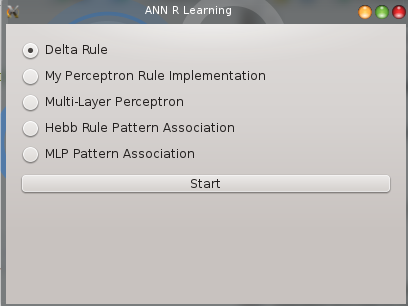
\includegraphics[width=\linewidth]{maingui.png}
 \caption{Main Interface} 
 
 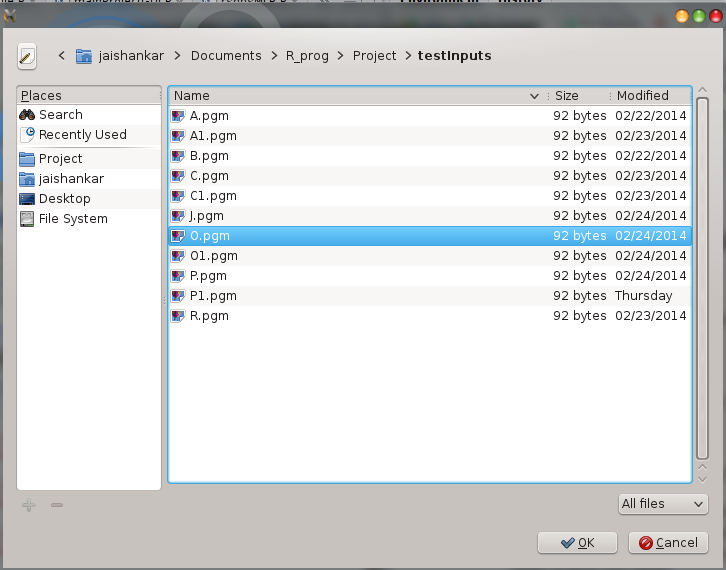
\includegraphics[width=\linewidth]{choosefile.png}
 \caption{Choosing a File} 
 \end{figure}
 
\newgeometry{margin=1cm}
\begin{landscape}
 \begin{figure}
 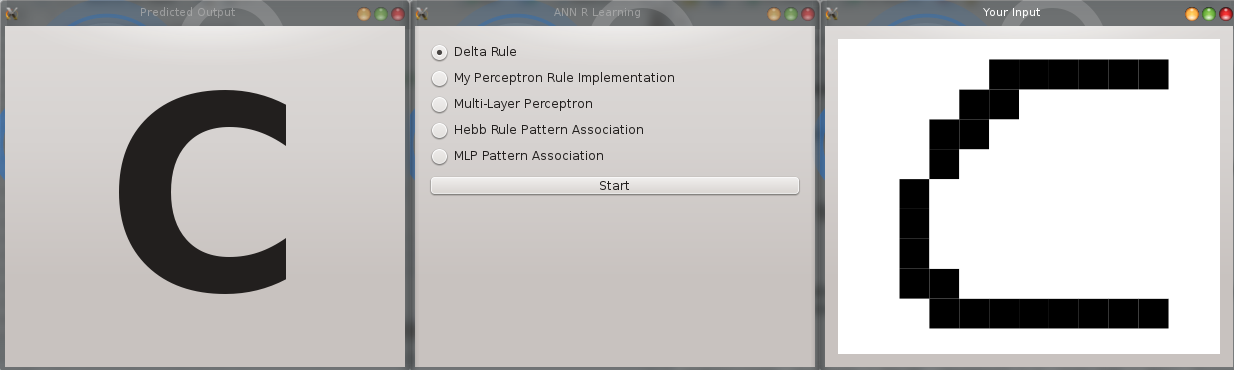
\includegraphics[width=\linewidth]{classificationoutput.png}
 \caption{Output of classification} 
 
 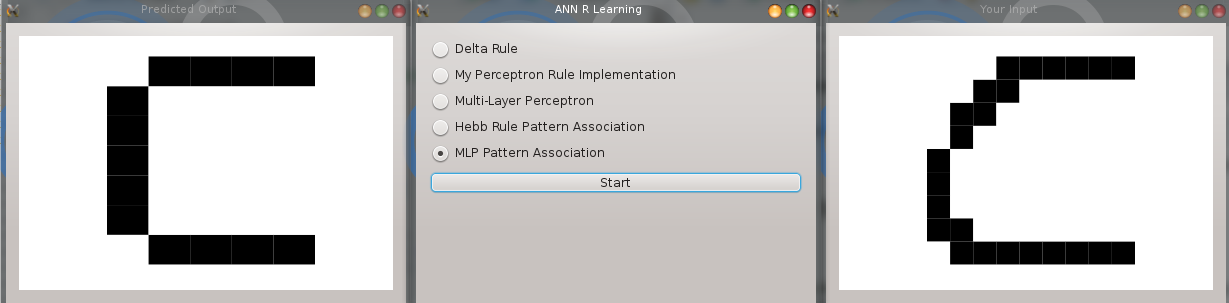
\includegraphics[width=\linewidth]{associationoutput.png}
 \caption{Output of Association} 
 \end{figure}
\end{landscape}
\restoregeometry
%show pctures about pattern association and then talk of different rules being implemented .. then the package implementation
%then gui code
%

\section*{R Code}
\addcontentsline{toc}{section}{R Code}
\subsubsection*{neuronClass.R}
This file contains the class that defines the basic structure of a neuron and all its basic properties. The methods that are defined in this file help manipulate the properties.
\begin{verbatim}
 neuron <- setClass("neuron",representation(weights="numeric",inputSignals="numeric",netInput="numeric",threshold="numeric",netOutput="numeric",bias="numeric"))
setInputSignals<-function(neuron, inputSignals)
{
  neuron@inputSignals<-inputSignals;
  return(neuron);
}
setWeights<-function(neuron, weights)
{
  neuron@inputSignals<-inputSignals;
  return(neuron);
}
intialise<-function(neuron, bias,threshold,weights,inputSignals)
{
  neuron@bias<-bias;
  neuron@threshold<-threshold;
  neuron@weights<-weights;
  neuron@inputSignals<-inputSignals;
}
calculateNetInput<-function(neuron)
{
  neuron@netInput <- sum(neuron@weights * neuron@inputSignals) + neuron@bias;
  return(neuron);
}
calculateNetOutput<-function(neuron)
{
  if(neuron@netInput > neuron@threshold)
  {
    neuron@netOutput = 1;
  }
  else if(neuron@netInput < (0-neuron@threshold))
  {
    neuron@netOutput = -1;
  }
  else
  {
    neuron@netOutput = 0;
  }
  return(neuron);
}
learn<-function(neuron, target)
{
  if(target != neuron@netOutput)
  {
    neuron@bias = neuron@bias + target;
    neuron@weights <- neuron@weights + target * neuron@inputSignals;
    return(neuron);
  }
  
  return(neuron);
}

\end{verbatim}

\subsubsection*{hiddenLayer.R}
This file defines the hidden layer, and all the neurons in it as objects of the class previously defined.

\begin{verbatim}
 
source("./neuronClass.R")

targetChars<-c("A","B","C","D","E","F","G","H","I","J",
  "K","L","M","N","O","P","Q","R","S","T","U","V","W","X","Y","Z")
hiddenLayer<-vector("list",length=noOutputUnits)

initialiseHiddenLayer<-function(hidden,trainingInputs)
{
  for(i in seq(1,noOutputUnits,1))
  {
    hidden[i]<-neuron(bias=0,weights=c(rep(0,noInputUnits)),
    inputSignals=trainingInputs,threshold=0,netInput=0,netOutput=0)
  }
  return(hidden);
}

\end{verbatim}

\subsubsection*{readFromPgmFile.R}
This file contains the code which encodes the \verb+.pgm+ image supplied by the user for prediction into a suitable binary representation, so that 
it can be fed into the network as input.
\begin{verbatim}
 #a main required file that scans the test input given by the user..
#the user is supposed to input a .pgm file...that is a pic file 
##using the pixmap package and the read.pnm we read the file and extract its inputs from the grey components of the image
require(gWidgets)
require(pixmap)
require(stringr)
options("guiToolkit"="RGtk2")
picfile<-gfile()

print(picfile)
found<-str_locate(picfile,".pgm")
assign("inputPredict",c())
if(is.na(found[1]))
{
  msg<-"Sorry Invalid File Input. Please restart the program and choose another file!"
  gmessage(msg,title="Invalid File", handler=function(h,...){return()})
}
  pix <- read.pnm(picfile)
  grey<-pix@grey
  inputPredict<-as.vector(t(grey)) #to get the matrix into a one dimensional vector...t() is for transpose.. transpose is necessary..otherwise the one dimensional vector does not come as expected
  inputPredict[which(inputPredict==1)]<--1
  inputPredict[which(inputPredict==0)]<-1
  ##the above vector inputPredict is the main converted vector that contains the properly converted input from black and white pixels into a bi-polar input vector for processing

\end{verbatim}

\subsubsection*{scanTrainingInputsFromFiles.R}
All the inputs and targets lists are populated in this file. The images that are pre-defined and drawn are read and 
converted into suitable bi-polar representation. The paths are hard-coded in this file, which need to be modified.
\begin{verbatim}
 ##this is one of the most required files..this file scans all the inputs and stores a lot of global variables that are used by many scripts..
## the input is got from pre drawn image .pgm files that I have drawn...they are considered to be targets and input for training
##first inputs are got....then targets(for classification),....then targets (for pattern association)
require(stringr)

require(pixmap)
setwd("/home/jaishankar/Documents/R_prog/Project/letters/")
##get the files
picfiles<-list.files()
print(picfiles)
trainingInputs<-list();
targets<-list();
noOutputUnits<- 26;
noTrainingInputs<-52;
noInputUnits<-81;
noAssocOutputUnits<-35
noAssocTrainingTargets<-26
##read and convert input to bipolar form
for(i in 1:length(picfiles))
{
  picfile<-picfiles[i]
  found<-str_locate(picfile,".pgm")
  if(is.na(found[1]))
  {
    msg<-"Sorry Invalid File Input. Please restart the program and choose another file!"
    gmessage(msg,title="Invalid File", handler=function(h,...){return()})
  }else
  {
    x <- read.pnm(picfile)
    
    grey<-x@grey
    input<-as.vector(t(grey)) #to get the matrix into a one dimensional vector...t() is for transpose.. transpose is necessary..otherwise the one dimensional vector does not come as expected
    ##the values in input which contain 1 are converted to -1 because in the .pgm 1 is stored as the value for which the pixel is off and 0 is the value for which the pixel is on...
    input[which(input==1)]=-1
    input[which(input==0)]=1
    trainingInputs[[i]]<-input
    t<-c(rep(-1,noOutputUnits));
    t[i] = 1;
    targets[[i]]<-t;
  }
}
setwd("/home/jaishankar/Documents/R_prog/Project/newletters/")
picfiles<-list.files()
len<-length(picfiles)
for(i in 1:len)
{
  picfile<-picfiles[i]
  found<-str_locate(picfile,".pgm")
  if(is.na(found[1]))
  {
    msg<-"Sorry Invalid File Input. Please restart the program and choose another file!"
    gmessage(msg,title="Invalid File", handler=function(h,...){return()})
  }else
  {
    x <- read.pnm(picfile)
   
    grey<-x@grey
    input<-as.vector(t(grey)) #to get the matrix into a one dimensional vector...t() is for transpose.. transpose is necessary..otherwise the one dimensional vector does not come as expected
    input[which(input==1)]=-1
    input[which(input==0)]=1
    trainingInputs[[i+len]]<-input
    t<-c(rep(-1,noOutputUnits));
    t[i] = 1;
    targets[[i+len]]<-t;
  }
}
setwd("/home/jaishankar/Documents/R_prog/Project/HebbTrainingnetwork/HebbTargets/")
picfiles<-list.files()
assocTargets<-list();

for(i in 1:length(picfiles))
{
  picfile<-picfiles[i]
  found<-str_locate(picfile,".pgm")
  if(is.na(found[1]))
  {
    msg<-"Sorry Invalid File Input. Please restart the program and choose another file!"
    gmessage(msg,title="Invalid File", handler=function(h,...){return()})
  }else
  {
    x <- read.pnm(picfile)
    
    grey<-x@grey
    input<-as.vector(t(grey)) #to get the matrix into a one dimensional vector...t() is for transpose.. transpose is necessary..otherwise the one dimensional vector does not come as expected
    input[which(input==1)]=-1
    input[which(input==0)]=1
    assocTargets[[i]]<-input
    
  }
}

##doing this restoring of the directory is very crucial to the working of the rest of the script..because the source command used in other scripts depend on this

setwd("/home/jaishankar/Documents/R_prog/Project")
\end{verbatim}

\subsubsection*{mainProjectGUI.R}
This is the main file that calls or sources all the other files. This file also presents the main GUI to the user, 
gets his input and sources the correct file for training and prediction. Again the paths are absolute paths that are
hard-coded and need modification.
\begin{verbatim}
 ##main gui and source file that essentially calls all the other files...contains some of the important global defintions
##the XXXXError variables are important for error plotting

require(gWidgets)
setwd("/home/jaishankar/Documents/R_prog/Project")
options("guiToolkit"="RGtk2")
deltaError<-c();
perceptronError<-c()
myPerceptronError<-c()
hebbError<-c()

mlpTrained=FALSE
deltaTrained=FALSE
mymlpTrained=FALSE
hebbTrained=FALSE
mplpatternTrained=FALSE
mainWindow<-gwindow("ANN R Learning")
mainGroup<-ggroup(horizontal=FALSE,container=mainWindow)
trainingGroup<-ggroup(container=mainGroup)
trainSelect <- gradio(c("Delta Rule","My Perceptron Rule Implementation","Multi-Layer Perceptron","Hebb Rule Pattern Association","MLP Pattern Association"), container=trainingGroup)
targetChars<-c("A","B","C","D","E","F","G","H","I","J","K","L","M","N","O","P","Q","R","S","T","U","V","W","X","Y","Z")


##function that handles the click in the gui...
##depending the choice sources the correct file and performs the learning only once by setting and checking a boolean variable XXXXtrained...
##finally the output display will depend on the predictedoutput which is defined and set in all the corresponding files...
startDemo<-function(h,...)
{
  rule<-svalue(trainSelect);
  if(is.na(rule))
  {
    msg<-"Sorry Choose a Rule to start with"
    gmessage(msg,title="Invalid Choice", handler=function(h,...){return()},parent=mainWindow)
  }
  source("./readFromPgmfile.R")
  source("./scanTrainingInputsFromFiles.R")
  if(rule == "My Perceptron Rule Implementation")
  {
    if(!mymlpTrained)
    {
      mlptime <<- proc.time()
      source("./maintrainingnetwork.R");
      mymlpTrained<<-TRUE;
      mlptime<-proc.time() - mlptime
      print(mlptime)
    }
    predictedoutput<-predict(hidden,inputPredict);
  }
  else if(rule == "Multi-Layer Perceptron")
  {
    if(!mlpTrained)
    {
      mlptime <<- proc.time()
      source("./rsnnsMLP.R");
      mlpTrained<<-TRUE;
      mlptime<-proc.time() - mlptime
      print(mlptime)
    }  
    test<-matrix(inputPredict,nrow=1)
    test[which(test==-1)]<-0
    predictedoutput<-predict.rsnns(model,test)
    print(predictedoutput)
    predictedoutput<-round(predictedoutput)
    
  }
  else if(rule == "Delta Rule")
  {
    if(!deltaTrained)
    {
      mlptime <<- proc.time()
      source("./DeltaLearningRule/maintrainingnetwork.R");
      deltaTrained<<-TRUE;
      mlptime<-proc.time() - mlptime
      print(mlptime)
    }
    predictedoutput<-predict(hidden,inputPredict);
  }
  else if(rule == "Hebb Rule Pattern Association")
  {
    if(!hebbTrained)
    {
      mlptime <<- proc.time()
      source("./HebbTrainingnetwork/hebbTrainingNetwork2.R");
      hebbTrained<<-TRUE;
      mlptime<-proc.time() - mlptime
      print(mlptime)
    }
    r<-c();
    ip<-inputPredict
    for(i in 1:ncol(weightVector))
    {
      r[i]<-sum(weightVector[,i]*ip);
      if(r[i]>0)
      {
        r[i]=0
      }
      else
      {
        r[i]=1
      }
    }
    
    print(r)
    p1<-matrix(r,nrow=7,byrow=TRUE)
    print(p1)
    respix<-pixmapGrey(p1,nrow=7,ncol=5,bbox=c(-1,-1,1,1))
    resultWindow<-gwindow("Predicted Output");
    
    ggraphics(width=250,height=150,ps=3, container=resultWindow)
    ##the sleep below is so that the ggraphics loads completely and fully before the plot command is called..else the plot command throws an error because there is no space to plot anything...
    Sys.sleep(2)
    plot(respix)
    ##this is called so that the plotting happens on the gui instead of some other output
    ggraphics(width=250,height=150,ps=3, container=gwindow("Your Input"))
    Sys.sleep(2)
    plot(pix)
    print(r)
    return();
  }
  else if(rule == "MLP Pattern Association")
  {
    if(!mplpatternTrained)
    {
      mlptime <<- proc.time()
      source("./MLP_pattern_asscociation/rsnnsMPLpatternAssoc.R");
      mplpatternTrained<<-TRUE;
      mlptime<-proc.time() - mlptime
      print(mlptime)
    }
    test<-matrix(inputPredict,nrow=1)
    test[which(test==-1)]<-0
    predictedoutput<-predict.rsnns(model,test)
    print(predictedoutput)
    predictedoutput<-round(predictedoutput)
    predictedoutput[which(predictedoutput==1)]<--1
    predictedoutput[which(predictedoutput==0)]<-1
    predictedoutput[which(predictedoutput==-1)]<-0
    r<-predictedoutput;
    p1<-matrix(r,nrow=7,byrow=TRUE)
    respix<-pixmapGrey(p1,nrow=7,ncol=5,bbox=c(-1,-1,1,1))
    resultWindow<-gwindow("Predicted Output");
    
    ggraphics(width=250,height=150,ps=3, container=resultWindow)
    
    Sys.sleep(2)
    plot(respix)
    ggraphics(width=250,height=150,ps=3, container=gwindow("Your Input"))
    Sys.sleep(2)
    plot(pix)
    print(r)
    return();
    }
  else
  {
    msg<-"Sorry that rule is not yet Implemented!!"
    gmessage(msg,title="Invalid Choice", handler=function(h,...){return()},parent=mainWindow)
  }
  print(predictedoutput);
  index<-which(predictedoutput==1);
  writeLines(targetChars[index]);
  charToPrint<-targetChars[index];
  if(!any(predictedoutput==1))
  {
    charToPrint<-"Sorry Could Not Guess!!"
  }
  resultWindow<-gwindow("Your Input");
  #group<-ggroup(horizontal=FALSE,container=resultWindow)
  ggraphics(width=250,height=150,ps=3, container=resultWindow)
  Sys.sleep(2)
  label<-glabel(charToPrint,container=gwindow("Predicted Output"))
  font(label)<- list(family="times",size=200,weight="bold",style="bold")
  plot(pix)
  
}
startButton<-gbutton("Start",container=mainGroup,handler=startDemo);
\end{verbatim}

\subsubsection*{rsnnsMLP.R}
This file makes use of the RSNNS package's \verb+mlp+ function to train the multi-layer perceptron.

\begin{verbatim}
 #this package is required for the mlp network to function
require(RSNNS)

#the training inputs and targets need to be in matrix form..whereas the inputs and targets scanned from the file are put into a list so we need to convert them...because the mlp expects it that way...

mlpTrainingInputs<-matrix(nrow=noTrainingInputs,ncol=noInputUnits)
mlpTrainingTargets<-matrix(nrow=noTrainingInputs,ncol=noOutputUnits)
#the matrix is modeled in such a way that the columns present the different inputs to a single training input
#where as the rows indicate the different training inputs presented for training..
for(i in 1:length(trainingInputs))
{
  mlpTrainingInputs[i,]<-trainingInputs[[i]];
  mlpTrainingInputs[which(mlpTrainingInputs==-1)]=0;
  mlpTrainingTargets[i,]<-targets[[i]];
  mlpTrainingTargets[which(mlpTrainingTargets==-1)]=0;
}
ml<-splitForTrainingAndTest(mlpTrainingInputs, mlpTrainingTargets, ratio = 0.15)

# model<-mlp(mlpTrainingInputs,mlpTrainingTargets,size=c(noOutputUnits),
#            hiddenActFunc = "Act_Logistic", learnFuncParams = c(0.4, 0.0),
#            learnFunc = "Std_Backpropagation")
##main class/function that trains the mlp(multi layer perceptron) and returns the trained model... which is used in the prediction
model<-mlp(ml$inputsTrain,ml$targetsTrain,size=noOutputUnits,
           learnFuncParams = 0.1, maxit = 3000, inputsTest = ml$inputsTest,
						targetsTest = ml$targetsTest)


\end{verbatim}





\begin{thebibliography}{9}

  \bibitem{wikiocr}
  Wikipedia, \url{http://en.wikipedia.org/wiki/Optical_character_recognition}
  \bibitem{fig1}Figure 1 \url{http://gigaom2.files.wordpress.com/2013/08/1000px-artificial_neural_network-svg.png}
  \bibitem{bookann} Book {Fundamentals of Neural Networks (Laurene Fausett)}
  \bibitem{cite_key2} {Neural Networks in R Using the Stuttgart Neural Network Simulator: RSNNS}
  \bibitem{cite_key3} {Packages manual pages}
  \bibitem{cite_key4} {Introduction to Neural Networks using MATLAB}
  

\end{thebibliography}

\end{document}          
